% backtracking worksheet template
\documentclass[leqno, 12pt]{article}
\usepackage{tikz}  
\usetikzlibrary{positioning}
\usetikzlibrary {arrows.meta}
\usepackage[a4paper, portrait, margin=1cm]{geometry}
\usepackage{multicol}
\usepackage{fancyhdr}


\tikzset{backtrack/.style={rectangle,draw=black,fill=white,
inner sep=2pt,minimum height=32pt, minimum width=20mm}}
\tikzset{backtrackeq/.style={rectangle,draw=black,fill=white,
inner sep=2pt,minimum height=12pt, minimum width=20mm}}
\tikzset{backtrackstep/.style={rectangle,draw=none,fill=white,
inner sep=2pt,minimum height=12pt, minimum width=20mm}}

\def \HeadingQuestions {\section*{\Large Name: \underline{\hspace{8cm}} \hfill Date: \underline{\hspace{3cm}}} \vspace{-3mm}
{2-step backtracking: Questions} \vspace{1pt}\hrule}

% raise footer with page number
\fancypagestyle{myfancypagestyle}{
  \fancyhf{} % clear all header and footer fields
  \renewcommand{\headrulewidth}{0pt} % no rule under header
  \fancyfoot[C] {\thepage} \setlength{\footskip}{6pt} % raise page number 6pt
}
\pagestyle{myfancypagestyle}  % apply myfancypagestyle


\begin{document}
    \HeadingQuestions
    \vspace{-8mm}
    \begin{multicols}{2}
        \begin{equation}
    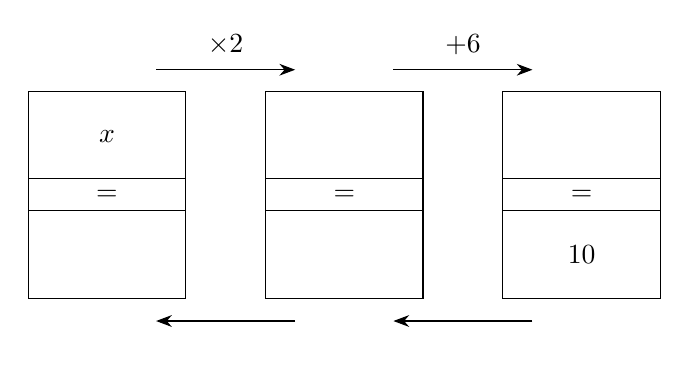
\begin{tikzpicture}[baseline={([yshift=-12pt]current bounding box.north)}]
            
        \node[backtrack] (boxA) at (0, 0) {$x$};
        \node[backtrack] (boxB) [right=1cm of boxA] {$$};
        \node[backtrack] (boxC) [right=1cm of boxB] {$$};
    
        \node[backtrackeq] (boxAeq) [below=-1pt of boxA] {$=$};
        \node[backtrackeq] (boxBeq) [below=-1pt of boxB] {$=$};
        \node[backtrackeq] (boxCeq) [below=-1pt of boxC] {$=$};
        
        \node[backtrack] (boxArev) [below=-1pt of boxAeq] {$$};
        \node[backtrack] (boxBrev) [below=-1pt of boxBeq] {$$};
        \node[backtrack] (boxCrev) [below=-1pt of boxCeq] {$10$};
         
        \node (boxAr) at ([yshift=24pt,xshift=5mm]boxA) { };
        \node (boxBl) at ([yshift=24pt,xshift=-5mm]boxB) { };
        \draw [line width=0.4pt,-{Stealth[length=2mm]}] (boxAr)  --node[backtrackstep, above=3.0pt] {$\times2$} (boxBl);
    
        \node (boxBr) at ([yshift=24pt,xshift=5mm]boxB) { };
        \node (boxCl) at ([yshift=24pt,xshift=-5mm]boxC) { };
        \draw [line width=0.4pt,-{Stealth[length=2mm]}] (boxBr)  --node[backtrackstep, above=3.0pt] {$+6$} (boxCl);
    
        \node (boxCrevl) at ([yshift=-24pt,xshift=-5mm]boxCrev) { };
        \node (boxBrevr) at ([yshift=-24pt,xshift=5mm]boxBrev) { };
        \draw [line width=0.4pt,-{Stealth[length=2mm]}] (boxCrevl)  --node[backtrackstep, below=3.0pt] {$$} (boxBrevr);
    
        \node (boxBrevl) at ([yshift=-24pt,xshift=-5mm]boxBrev) { };
        \node (boxArevr) at ([yshift=-24pt,xshift=5mm]boxArev) { };
        \draw [line width=0.4pt,-{Stealth[length=2mm]}] (boxBrevl)  --node[backtrackstep, below=3.0pt] {$$} (boxArevr);
        
    \end{tikzpicture}    
\end{equation}


\vspace{-2pt}\begin{equation}
    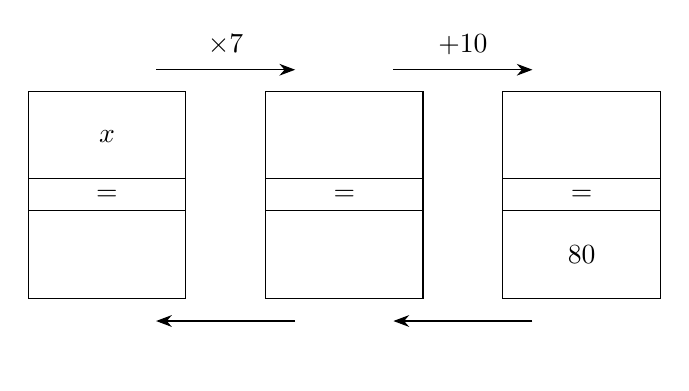
\begin{tikzpicture}[baseline={([yshift=-12pt]current bounding box.north)}]
            
        \node[backtrack] (boxA) at (0, 0) {$x$};
        \node[backtrack] (boxB) [right=1cm of boxA] {$$};
        \node[backtrack] (boxC) [right=1cm of boxB] {$$};
    
        \node[backtrackeq] (boxAeq) [below=-1pt of boxA] {$=$};
        \node[backtrackeq] (boxBeq) [below=-1pt of boxB] {$=$};
        \node[backtrackeq] (boxCeq) [below=-1pt of boxC] {$=$};
        
        \node[backtrack] (boxArev) [below=-1pt of boxAeq] {$$};
        \node[backtrack] (boxBrev) [below=-1pt of boxBeq] {$$};
        \node[backtrack] (boxCrev) [below=-1pt of boxCeq] {$80$};
         
        \node (boxAr) at ([yshift=24pt,xshift=5mm]boxA) { };
        \node (boxBl) at ([yshift=24pt,xshift=-5mm]boxB) { };
        \draw [line width=0.4pt,-{Stealth[length=2mm]}] (boxAr)  --node[backtrackstep, above=3.0pt] {$\times7$} (boxBl);
    
        \node (boxBr) at ([yshift=24pt,xshift=5mm]boxB) { };
        \node (boxCl) at ([yshift=24pt,xshift=-5mm]boxC) { };
        \draw [line width=0.4pt,-{Stealth[length=2mm]}] (boxBr)  --node[backtrackstep, above=3.0pt] {$+10$} (boxCl);
    
        \node (boxCrevl) at ([yshift=-24pt,xshift=-5mm]boxCrev) { };
        \node (boxBrevr) at ([yshift=-24pt,xshift=5mm]boxBrev) { };
        \draw [line width=0.4pt,-{Stealth[length=2mm]}] (boxCrevl)  --node[backtrackstep, below=3.0pt] {$$} (boxBrevr);
    
        \node (boxBrevl) at ([yshift=-24pt,xshift=-5mm]boxBrev) { };
        \node (boxArevr) at ([yshift=-24pt,xshift=5mm]boxArev) { };
        \draw [line width=0.4pt,-{Stealth[length=2mm]}] (boxBrevl)  --node[backtrackstep, below=3.0pt] {$$} (boxArevr);
        
    \end{tikzpicture}    
\end{equation}


\vspace{-2pt}\begin{equation}
    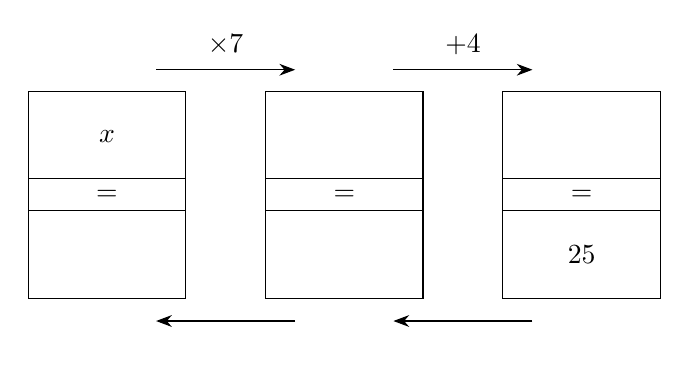
\begin{tikzpicture}[baseline={([yshift=-12pt]current bounding box.north)}]
            
        \node[backtrack] (boxA) at (0, 0) {$x$};
        \node[backtrack] (boxB) [right=1cm of boxA] {$$};
        \node[backtrack] (boxC) [right=1cm of boxB] {$$};
    
        \node[backtrackeq] (boxAeq) [below=-1pt of boxA] {$=$};
        \node[backtrackeq] (boxBeq) [below=-1pt of boxB] {$=$};
        \node[backtrackeq] (boxCeq) [below=-1pt of boxC] {$=$};
        
        \node[backtrack] (boxArev) [below=-1pt of boxAeq] {$$};
        \node[backtrack] (boxBrev) [below=-1pt of boxBeq] {$$};
        \node[backtrack] (boxCrev) [below=-1pt of boxCeq] {$25$};
         
        \node (boxAr) at ([yshift=24pt,xshift=5mm]boxA) { };
        \node (boxBl) at ([yshift=24pt,xshift=-5mm]boxB) { };
        \draw [line width=0.4pt,-{Stealth[length=2mm]}] (boxAr)  --node[backtrackstep, above=3.0pt] {$\times7$} (boxBl);
    
        \node (boxBr) at ([yshift=24pt,xshift=5mm]boxB) { };
        \node (boxCl) at ([yshift=24pt,xshift=-5mm]boxC) { };
        \draw [line width=0.4pt,-{Stealth[length=2mm]}] (boxBr)  --node[backtrackstep, above=3.0pt] {$+4$} (boxCl);
    
        \node (boxCrevl) at ([yshift=-24pt,xshift=-5mm]boxCrev) { };
        \node (boxBrevr) at ([yshift=-24pt,xshift=5mm]boxBrev) { };
        \draw [line width=0.4pt,-{Stealth[length=2mm]}] (boxCrevl)  --node[backtrackstep, below=3.0pt] {$$} (boxBrevr);
    
        \node (boxBrevl) at ([yshift=-24pt,xshift=-5mm]boxBrev) { };
        \node (boxArevr) at ([yshift=-24pt,xshift=5mm]boxArev) { };
        \draw [line width=0.4pt,-{Stealth[length=2mm]}] (boxBrevl)  --node[backtrackstep, below=3.0pt] {$$} (boxArevr);
        
    \end{tikzpicture}    
\end{equation}


\vspace{-2pt}\begin{equation}
    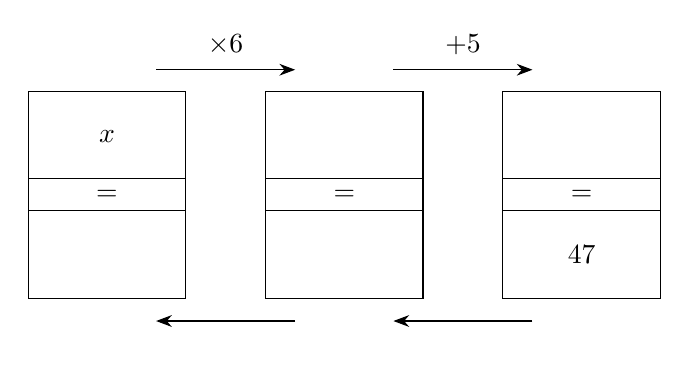
\begin{tikzpicture}[baseline={([yshift=-12pt]current bounding box.north)}]
            
        \node[backtrack] (boxA) at (0, 0) {$x$};
        \node[backtrack] (boxB) [right=1cm of boxA] {$$};
        \node[backtrack] (boxC) [right=1cm of boxB] {$$};
    
        \node[backtrackeq] (boxAeq) [below=-1pt of boxA] {$=$};
        \node[backtrackeq] (boxBeq) [below=-1pt of boxB] {$=$};
        \node[backtrackeq] (boxCeq) [below=-1pt of boxC] {$=$};
        
        \node[backtrack] (boxArev) [below=-1pt of boxAeq] {$$};
        \node[backtrack] (boxBrev) [below=-1pt of boxBeq] {$$};
        \node[backtrack] (boxCrev) [below=-1pt of boxCeq] {$47$};
         
        \node (boxAr) at ([yshift=24pt,xshift=5mm]boxA) { };
        \node (boxBl) at ([yshift=24pt,xshift=-5mm]boxB) { };
        \draw [line width=0.4pt,-{Stealth[length=2mm]}] (boxAr)  --node[backtrackstep, above=3.0pt] {$\times6$} (boxBl);
    
        \node (boxBr) at ([yshift=24pt,xshift=5mm]boxB) { };
        \node (boxCl) at ([yshift=24pt,xshift=-5mm]boxC) { };
        \draw [line width=0.4pt,-{Stealth[length=2mm]}] (boxBr)  --node[backtrackstep, above=3.0pt] {$+5$} (boxCl);
    
        \node (boxCrevl) at ([yshift=-24pt,xshift=-5mm]boxCrev) { };
        \node (boxBrevr) at ([yshift=-24pt,xshift=5mm]boxBrev) { };
        \draw [line width=0.4pt,-{Stealth[length=2mm]}] (boxCrevl)  --node[backtrackstep, below=3.0pt] {$$} (boxBrevr);
    
        \node (boxBrevl) at ([yshift=-24pt,xshift=-5mm]boxBrev) { };
        \node (boxArevr) at ([yshift=-24pt,xshift=5mm]boxArev) { };
        \draw [line width=0.4pt,-{Stealth[length=2mm]}] (boxBrevl)  --node[backtrackstep, below=3.0pt] {$$} (boxArevr);
        
    \end{tikzpicture}    
\end{equation}


\vspace{-2pt}\begin{equation}
    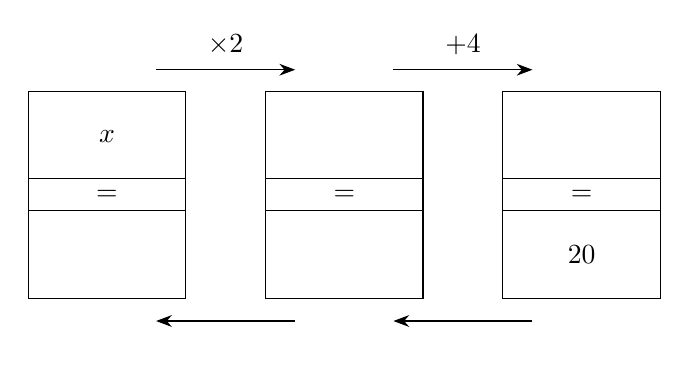
\begin{tikzpicture}[baseline={([yshift=-12pt]current bounding box.north)}]
            
        \node[backtrack] (boxA) at (0, 0) {$x$};
        \node[backtrack] (boxB) [right=1cm of boxA] {$$};
        \node[backtrack] (boxC) [right=1cm of boxB] {$$};
    
        \node[backtrackeq] (boxAeq) [below=-1pt of boxA] {$=$};
        \node[backtrackeq] (boxBeq) [below=-1pt of boxB] {$=$};
        \node[backtrackeq] (boxCeq) [below=-1pt of boxC] {$=$};
        
        \node[backtrack] (boxArev) [below=-1pt of boxAeq] {$$};
        \node[backtrack] (boxBrev) [below=-1pt of boxBeq] {$$};
        \node[backtrack] (boxCrev) [below=-1pt of boxCeq] {$20$};
         
        \node (boxAr) at ([yshift=24pt,xshift=5mm]boxA) { };
        \node (boxBl) at ([yshift=24pt,xshift=-5mm]boxB) { };
        \draw [line width=0.4pt,-{Stealth[length=2mm]}] (boxAr)  --node[backtrackstep, above=3.0pt] {$\times2$} (boxBl);
    
        \node (boxBr) at ([yshift=24pt,xshift=5mm]boxB) { };
        \node (boxCl) at ([yshift=24pt,xshift=-5mm]boxC) { };
        \draw [line width=0.4pt,-{Stealth[length=2mm]}] (boxBr)  --node[backtrackstep, above=3.0pt] {$+4$} (boxCl);
    
        \node (boxCrevl) at ([yshift=-24pt,xshift=-5mm]boxCrev) { };
        \node (boxBrevr) at ([yshift=-24pt,xshift=5mm]boxBrev) { };
        \draw [line width=0.4pt,-{Stealth[length=2mm]}] (boxCrevl)  --node[backtrackstep, below=3.0pt] {$$} (boxBrevr);
    
        \node (boxBrevl) at ([yshift=-24pt,xshift=-5mm]boxBrev) { };
        \node (boxArevr) at ([yshift=-24pt,xshift=5mm]boxArev) { };
        \draw [line width=0.4pt,-{Stealth[length=2mm]}] (boxBrevl)  --node[backtrackstep, below=3.0pt] {$$} (boxArevr);
        
    \end{tikzpicture}    
\end{equation}


\vspace{-2pt}\begin{equation}
    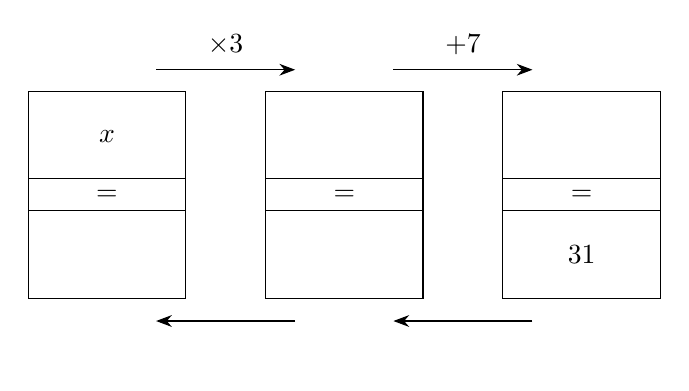
\begin{tikzpicture}[baseline={([yshift=-12pt]current bounding box.north)}]
            
        \node[backtrack] (boxA) at (0, 0) {$x$};
        \node[backtrack] (boxB) [right=1cm of boxA] {$$};
        \node[backtrack] (boxC) [right=1cm of boxB] {$$};
    
        \node[backtrackeq] (boxAeq) [below=-1pt of boxA] {$=$};
        \node[backtrackeq] (boxBeq) [below=-1pt of boxB] {$=$};
        \node[backtrackeq] (boxCeq) [below=-1pt of boxC] {$=$};
        
        \node[backtrack] (boxArev) [below=-1pt of boxAeq] {$$};
        \node[backtrack] (boxBrev) [below=-1pt of boxBeq] {$$};
        \node[backtrack] (boxCrev) [below=-1pt of boxCeq] {$31$};
         
        \node (boxAr) at ([yshift=24pt,xshift=5mm]boxA) { };
        \node (boxBl) at ([yshift=24pt,xshift=-5mm]boxB) { };
        \draw [line width=0.4pt,-{Stealth[length=2mm]}] (boxAr)  --node[backtrackstep, above=3.0pt] {$\times3$} (boxBl);
    
        \node (boxBr) at ([yshift=24pt,xshift=5mm]boxB) { };
        \node (boxCl) at ([yshift=24pt,xshift=-5mm]boxC) { };
        \draw [line width=0.4pt,-{Stealth[length=2mm]}] (boxBr)  --node[backtrackstep, above=3.0pt] {$+7$} (boxCl);
    
        \node (boxCrevl) at ([yshift=-24pt,xshift=-5mm]boxCrev) { };
        \node (boxBrevr) at ([yshift=-24pt,xshift=5mm]boxBrev) { };
        \draw [line width=0.4pt,-{Stealth[length=2mm]}] (boxCrevl)  --node[backtrackstep, below=3.0pt] {$$} (boxBrevr);
    
        \node (boxBrevl) at ([yshift=-24pt,xshift=-5mm]boxBrev) { };
        \node (boxArevr) at ([yshift=-24pt,xshift=5mm]boxArev) { };
        \draw [line width=0.4pt,-{Stealth[length=2mm]}] (boxBrevl)  --node[backtrackstep, below=3.0pt] {$$} (boxArevr);
        
    \end{tikzpicture}    
\end{equation}


\vspace{-2pt}\begin{equation}
    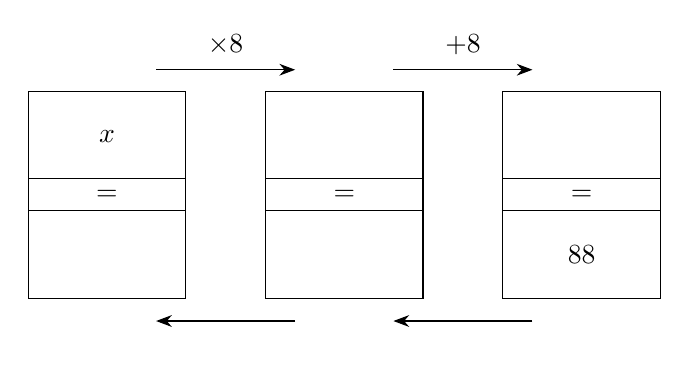
\begin{tikzpicture}[baseline={([yshift=-12pt]current bounding box.north)}]
            
        \node[backtrack] (boxA) at (0, 0) {$x$};
        \node[backtrack] (boxB) [right=1cm of boxA] {$$};
        \node[backtrack] (boxC) [right=1cm of boxB] {$$};
    
        \node[backtrackeq] (boxAeq) [below=-1pt of boxA] {$=$};
        \node[backtrackeq] (boxBeq) [below=-1pt of boxB] {$=$};
        \node[backtrackeq] (boxCeq) [below=-1pt of boxC] {$=$};
        
        \node[backtrack] (boxArev) [below=-1pt of boxAeq] {$$};
        \node[backtrack] (boxBrev) [below=-1pt of boxBeq] {$$};
        \node[backtrack] (boxCrev) [below=-1pt of boxCeq] {$88$};
         
        \node (boxAr) at ([yshift=24pt,xshift=5mm]boxA) { };
        \node (boxBl) at ([yshift=24pt,xshift=-5mm]boxB) { };
        \draw [line width=0.4pt,-{Stealth[length=2mm]}] (boxAr)  --node[backtrackstep, above=3.0pt] {$\times8$} (boxBl);
    
        \node (boxBr) at ([yshift=24pt,xshift=5mm]boxB) { };
        \node (boxCl) at ([yshift=24pt,xshift=-5mm]boxC) { };
        \draw [line width=0.4pt,-{Stealth[length=2mm]}] (boxBr)  --node[backtrackstep, above=3.0pt] {$+8$} (boxCl);
    
        \node (boxCrevl) at ([yshift=-24pt,xshift=-5mm]boxCrev) { };
        \node (boxBrevr) at ([yshift=-24pt,xshift=5mm]boxBrev) { };
        \draw [line width=0.4pt,-{Stealth[length=2mm]}] (boxCrevl)  --node[backtrackstep, below=3.0pt] {$$} (boxBrevr);
    
        \node (boxBrevl) at ([yshift=-24pt,xshift=-5mm]boxBrev) { };
        \node (boxArevr) at ([yshift=-24pt,xshift=5mm]boxArev) { };
        \draw [line width=0.4pt,-{Stealth[length=2mm]}] (boxBrevl)  --node[backtrackstep, below=3.0pt] {$$} (boxArevr);
        
    \end{tikzpicture}    
\end{equation}


\vspace{-2pt}\begin{equation}
    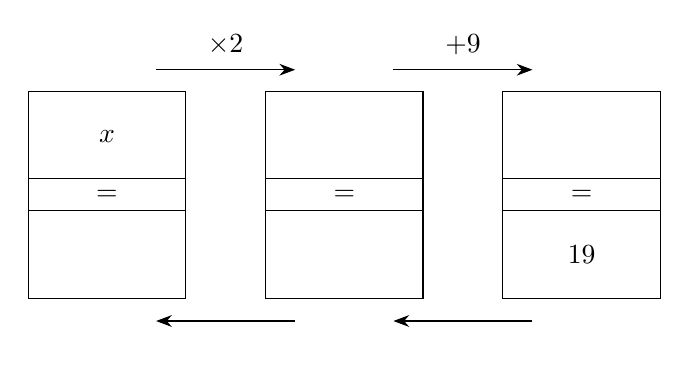
\begin{tikzpicture}[baseline={([yshift=-12pt]current bounding box.north)}]
            
        \node[backtrack] (boxA) at (0, 0) {$x$};
        \node[backtrack] (boxB) [right=1cm of boxA] {$$};
        \node[backtrack] (boxC) [right=1cm of boxB] {$$};
    
        \node[backtrackeq] (boxAeq) [below=-1pt of boxA] {$=$};
        \node[backtrackeq] (boxBeq) [below=-1pt of boxB] {$=$};
        \node[backtrackeq] (boxCeq) [below=-1pt of boxC] {$=$};
        
        \node[backtrack] (boxArev) [below=-1pt of boxAeq] {$$};
        \node[backtrack] (boxBrev) [below=-1pt of boxBeq] {$$};
        \node[backtrack] (boxCrev) [below=-1pt of boxCeq] {$19$};
         
        \node (boxAr) at ([yshift=24pt,xshift=5mm]boxA) { };
        \node (boxBl) at ([yshift=24pt,xshift=-5mm]boxB) { };
        \draw [line width=0.4pt,-{Stealth[length=2mm]}] (boxAr)  --node[backtrackstep, above=3.0pt] {$\times2$} (boxBl);
    
        \node (boxBr) at ([yshift=24pt,xshift=5mm]boxB) { };
        \node (boxCl) at ([yshift=24pt,xshift=-5mm]boxC) { };
        \draw [line width=0.4pt,-{Stealth[length=2mm]}] (boxBr)  --node[backtrackstep, above=3.0pt] {$+9$} (boxCl);
    
        \node (boxCrevl) at ([yshift=-24pt,xshift=-5mm]boxCrev) { };
        \node (boxBrevr) at ([yshift=-24pt,xshift=5mm]boxBrev) { };
        \draw [line width=0.4pt,-{Stealth[length=2mm]}] (boxCrevl)  --node[backtrackstep, below=3.0pt] {$$} (boxBrevr);
    
        \node (boxBrevl) at ([yshift=-24pt,xshift=-5mm]boxBrev) { };
        \node (boxArevr) at ([yshift=-24pt,xshift=5mm]boxArev) { };
        \draw [line width=0.4pt,-{Stealth[length=2mm]}] (boxBrevl)  --node[backtrackstep, below=3.0pt] {$$} (boxArevr);
        
    \end{tikzpicture}    
\end{equation}


\vspace{-2pt}\begin{equation}
    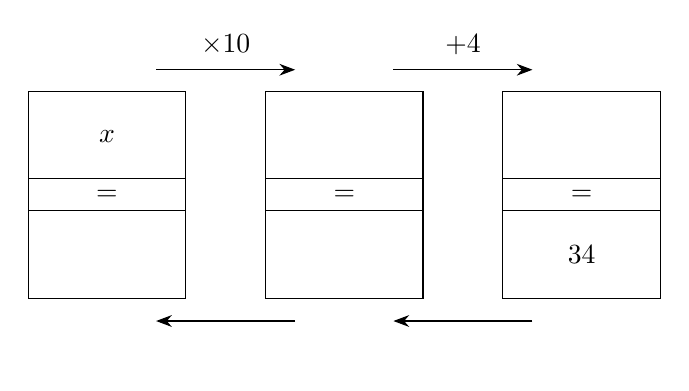
\begin{tikzpicture}[baseline={([yshift=-12pt]current bounding box.north)}]
            
        \node[backtrack] (boxA) at (0, 0) {$x$};
        \node[backtrack] (boxB) [right=1cm of boxA] {$$};
        \node[backtrack] (boxC) [right=1cm of boxB] {$$};
    
        \node[backtrackeq] (boxAeq) [below=-1pt of boxA] {$=$};
        \node[backtrackeq] (boxBeq) [below=-1pt of boxB] {$=$};
        \node[backtrackeq] (boxCeq) [below=-1pt of boxC] {$=$};
        
        \node[backtrack] (boxArev) [below=-1pt of boxAeq] {$$};
        \node[backtrack] (boxBrev) [below=-1pt of boxBeq] {$$};
        \node[backtrack] (boxCrev) [below=-1pt of boxCeq] {$34$};
         
        \node (boxAr) at ([yshift=24pt,xshift=5mm]boxA) { };
        \node (boxBl) at ([yshift=24pt,xshift=-5mm]boxB) { };
        \draw [line width=0.4pt,-{Stealth[length=2mm]}] (boxAr)  --node[backtrackstep, above=3.0pt] {$\times10$} (boxBl);
    
        \node (boxBr) at ([yshift=24pt,xshift=5mm]boxB) { };
        \node (boxCl) at ([yshift=24pt,xshift=-5mm]boxC) { };
        \draw [line width=0.4pt,-{Stealth[length=2mm]}] (boxBr)  --node[backtrackstep, above=3.0pt] {$+4$} (boxCl);
    
        \node (boxCrevl) at ([yshift=-24pt,xshift=-5mm]boxCrev) { };
        \node (boxBrevr) at ([yshift=-24pt,xshift=5mm]boxBrev) { };
        \draw [line width=0.4pt,-{Stealth[length=2mm]}] (boxCrevl)  --node[backtrackstep, below=3.0pt] {$$} (boxBrevr);
    
        \node (boxBrevl) at ([yshift=-24pt,xshift=-5mm]boxBrev) { };
        \node (boxArevr) at ([yshift=-24pt,xshift=5mm]boxArev) { };
        \draw [line width=0.4pt,-{Stealth[length=2mm]}] (boxBrevl)  --node[backtrackstep, below=3.0pt] {$$} (boxArevr);
        
    \end{tikzpicture}    
\end{equation}


\vspace{-2pt}\begin{equation}
    \begin{tikzpicture}[baseline={([yshift=-12pt]current bounding box.north)}]
            
        \node[backtrack] (boxA) at (0, 0) {$x$};
        \node[backtrack] (boxB) [right=1cm of boxA] {$$};
        \node[backtrack] (boxC) [right=1cm of boxB] {$$};
    
        \node[backtrackeq] (boxAeq) [below=-1pt of boxA] {$=$};
        \node[backtrackeq] (boxBeq) [below=-1pt of boxB] {$=$};
        \node[backtrackeq] (boxCeq) [below=-1pt of boxC] {$=$};
        
        \node[backtrack] (boxArev) [below=-1pt of boxAeq] {$$};
        \node[backtrack] (boxBrev) [below=-1pt of boxBeq] {$$};
        \node[backtrack] (boxCrev) [below=-1pt of boxCeq] {$61$};
         
        \node (boxAr) at ([yshift=24pt,xshift=5mm]boxA) { };
        \node (boxBl) at ([yshift=24pt,xshift=-5mm]boxB) { };
        \draw [line width=0.4pt,-{Stealth[length=2mm]}] (boxAr)  --node[backtrackstep, above=3.0pt] {$\times7$} (boxBl);
    
        \node (boxBr) at ([yshift=24pt,xshift=5mm]boxB) { };
        \node (boxCl) at ([yshift=24pt,xshift=-5mm]boxC) { };
        \draw [line width=0.4pt,-{Stealth[length=2mm]}] (boxBr)  --node[backtrackstep, above=3.0pt] {$+5$} (boxCl);
    
        \node (boxCrevl) at ([yshift=-24pt,xshift=-5mm]boxCrev) { };
        \node (boxBrevr) at ([yshift=-24pt,xshift=5mm]boxBrev) { };
        \draw [line width=0.4pt,-{Stealth[length=2mm]}] (boxCrevl)  --node[backtrackstep, below=3.0pt] {$$} (boxBrevr);
    
        \node (boxBrevl) at ([yshift=-24pt,xshift=-5mm]boxBrev) { };
        \node (boxArevr) at ([yshift=-24pt,xshift=5mm]boxArev) { };
        \draw [line width=0.4pt,-{Stealth[length=2mm]}] (boxBrevl)  --node[backtrackstep, below=3.0pt] {$$} (boxArevr);
        
    \end{tikzpicture}    
\end{equation}


\vspace{-2pt}\begin{equation}
    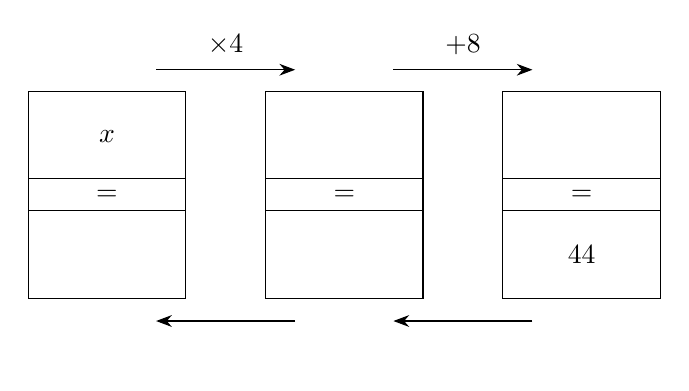
\begin{tikzpicture}[baseline={([yshift=-12pt]current bounding box.north)}]
            
        \node[backtrack] (boxA) at (0, 0) {$x$};
        \node[backtrack] (boxB) [right=1cm of boxA] {$$};
        \node[backtrack] (boxC) [right=1cm of boxB] {$$};
    
        \node[backtrackeq] (boxAeq) [below=-1pt of boxA] {$=$};
        \node[backtrackeq] (boxBeq) [below=-1pt of boxB] {$=$};
        \node[backtrackeq] (boxCeq) [below=-1pt of boxC] {$=$};
        
        \node[backtrack] (boxArev) [below=-1pt of boxAeq] {$$};
        \node[backtrack] (boxBrev) [below=-1pt of boxBeq] {$$};
        \node[backtrack] (boxCrev) [below=-1pt of boxCeq] {$44$};
         
        \node (boxAr) at ([yshift=24pt,xshift=5mm]boxA) { };
        \node (boxBl) at ([yshift=24pt,xshift=-5mm]boxB) { };
        \draw [line width=0.4pt,-{Stealth[length=2mm]}] (boxAr)  --node[backtrackstep, above=3.0pt] {$\times4$} (boxBl);
    
        \node (boxBr) at ([yshift=24pt,xshift=5mm]boxB) { };
        \node (boxCl) at ([yshift=24pt,xshift=-5mm]boxC) { };
        \draw [line width=0.4pt,-{Stealth[length=2mm]}] (boxBr)  --node[backtrackstep, above=3.0pt] {$+8$} (boxCl);
    
        \node (boxCrevl) at ([yshift=-24pt,xshift=-5mm]boxCrev) { };
        \node (boxBrevr) at ([yshift=-24pt,xshift=5mm]boxBrev) { };
        \draw [line width=0.4pt,-{Stealth[length=2mm]}] (boxCrevl)  --node[backtrackstep, below=3.0pt] {$$} (boxBrevr);
    
        \node (boxBrevl) at ([yshift=-24pt,xshift=-5mm]boxBrev) { };
        \node (boxArevr) at ([yshift=-24pt,xshift=5mm]boxArev) { };
        \draw [line width=0.4pt,-{Stealth[length=2mm]}] (boxBrevl)  --node[backtrackstep, below=3.0pt] {$$} (boxArevr);
        
    \end{tikzpicture}    
\end{equation}


\vspace{-2pt}\begin{equation}
    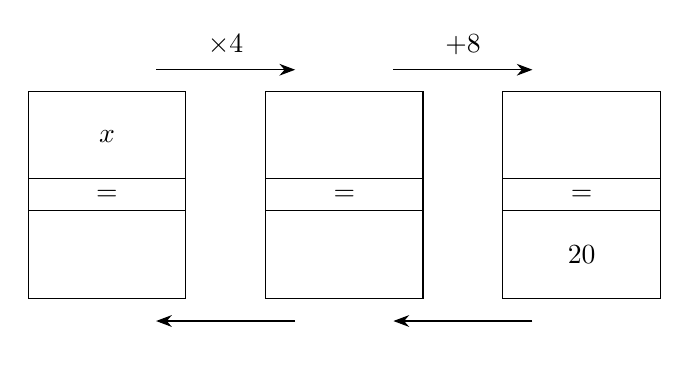
\begin{tikzpicture}[baseline={([yshift=-12pt]current bounding box.north)}]
            
        \node[backtrack] (boxA) at (0, 0) {$x$};
        \node[backtrack] (boxB) [right=1cm of boxA] {$$};
        \node[backtrack] (boxC) [right=1cm of boxB] {$$};
    
        \node[backtrackeq] (boxAeq) [below=-1pt of boxA] {$=$};
        \node[backtrackeq] (boxBeq) [below=-1pt of boxB] {$=$};
        \node[backtrackeq] (boxCeq) [below=-1pt of boxC] {$=$};
        
        \node[backtrack] (boxArev) [below=-1pt of boxAeq] {$$};
        \node[backtrack] (boxBrev) [below=-1pt of boxBeq] {$$};
        \node[backtrack] (boxCrev) [below=-1pt of boxCeq] {$20$};
         
        \node (boxAr) at ([yshift=24pt,xshift=5mm]boxA) { };
        \node (boxBl) at ([yshift=24pt,xshift=-5mm]boxB) { };
        \draw [line width=0.4pt,-{Stealth[length=2mm]}] (boxAr)  --node[backtrackstep, above=3.0pt] {$\times4$} (boxBl);
    
        \node (boxBr) at ([yshift=24pt,xshift=5mm]boxB) { };
        \node (boxCl) at ([yshift=24pt,xshift=-5mm]boxC) { };
        \draw [line width=0.4pt,-{Stealth[length=2mm]}] (boxBr)  --node[backtrackstep, above=3.0pt] {$+8$} (boxCl);
    
        \node (boxCrevl) at ([yshift=-24pt,xshift=-5mm]boxCrev) { };
        \node (boxBrevr) at ([yshift=-24pt,xshift=5mm]boxBrev) { };
        \draw [line width=0.4pt,-{Stealth[length=2mm]}] (boxCrevl)  --node[backtrackstep, below=3.0pt] {$$} (boxBrevr);
    
        \node (boxBrevl) at ([yshift=-24pt,xshift=-5mm]boxBrev) { };
        \node (boxArevr) at ([yshift=-24pt,xshift=5mm]boxArev) { };
        \draw [line width=0.4pt,-{Stealth[length=2mm]}] (boxBrevl)  --node[backtrackstep, below=3.0pt] {$$} (boxArevr);
        
    \end{tikzpicture}    
\end{equation}


\vspace{-2pt}\begin{equation}
    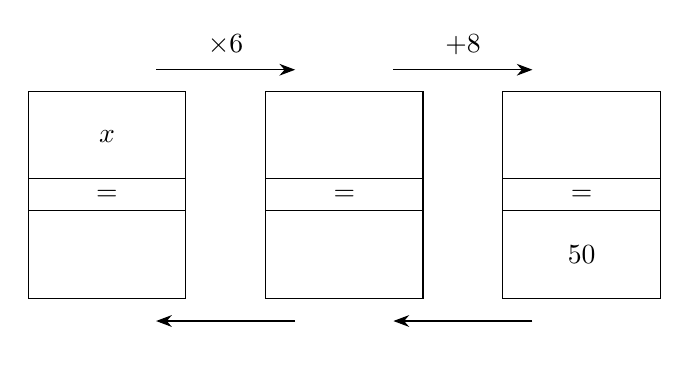
\begin{tikzpicture}[baseline={([yshift=-12pt]current bounding box.north)}]
            
        \node[backtrack] (boxA) at (0, 0) {$x$};
        \node[backtrack] (boxB) [right=1cm of boxA] {$$};
        \node[backtrack] (boxC) [right=1cm of boxB] {$$};
    
        \node[backtrackeq] (boxAeq) [below=-1pt of boxA] {$=$};
        \node[backtrackeq] (boxBeq) [below=-1pt of boxB] {$=$};
        \node[backtrackeq] (boxCeq) [below=-1pt of boxC] {$=$};
        
        \node[backtrack] (boxArev) [below=-1pt of boxAeq] {$$};
        \node[backtrack] (boxBrev) [below=-1pt of boxBeq] {$$};
        \node[backtrack] (boxCrev) [below=-1pt of boxCeq] {$50$};
         
        \node (boxAr) at ([yshift=24pt,xshift=5mm]boxA) { };
        \node (boxBl) at ([yshift=24pt,xshift=-5mm]boxB) { };
        \draw [line width=0.4pt,-{Stealth[length=2mm]}] (boxAr)  --node[backtrackstep, above=3.0pt] {$\times6$} (boxBl);
    
        \node (boxBr) at ([yshift=24pt,xshift=5mm]boxB) { };
        \node (boxCl) at ([yshift=24pt,xshift=-5mm]boxC) { };
        \draw [line width=0.4pt,-{Stealth[length=2mm]}] (boxBr)  --node[backtrackstep, above=3.0pt] {$+8$} (boxCl);
    
        \node (boxCrevl) at ([yshift=-24pt,xshift=-5mm]boxCrev) { };
        \node (boxBrevr) at ([yshift=-24pt,xshift=5mm]boxBrev) { };
        \draw [line width=0.4pt,-{Stealth[length=2mm]}] (boxCrevl)  --node[backtrackstep, below=3.0pt] {$$} (boxBrevr);
    
        \node (boxBrevl) at ([yshift=-24pt,xshift=-5mm]boxBrev) { };
        \node (boxArevr) at ([yshift=-24pt,xshift=5mm]boxArev) { };
        \draw [line width=0.4pt,-{Stealth[length=2mm]}] (boxBrevl)  --node[backtrackstep, below=3.0pt] {$$} (boxArevr);
        
    \end{tikzpicture}    
\end{equation}


\vspace{-2pt}\begin{equation}
    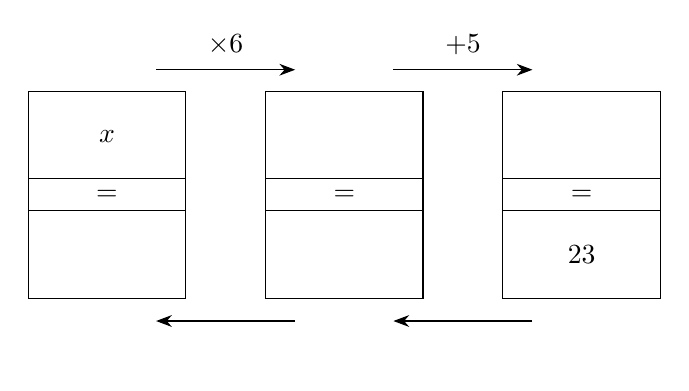
\begin{tikzpicture}[baseline={([yshift=-12pt]current bounding box.north)}]
            
        \node[backtrack] (boxA) at (0, 0) {$x$};
        \node[backtrack] (boxB) [right=1cm of boxA] {$$};
        \node[backtrack] (boxC) [right=1cm of boxB] {$$};
    
        \node[backtrackeq] (boxAeq) [below=-1pt of boxA] {$=$};
        \node[backtrackeq] (boxBeq) [below=-1pt of boxB] {$=$};
        \node[backtrackeq] (boxCeq) [below=-1pt of boxC] {$=$};
        
        \node[backtrack] (boxArev) [below=-1pt of boxAeq] {$$};
        \node[backtrack] (boxBrev) [below=-1pt of boxBeq] {$$};
        \node[backtrack] (boxCrev) [below=-1pt of boxCeq] {$23$};
         
        \node (boxAr) at ([yshift=24pt,xshift=5mm]boxA) { };
        \node (boxBl) at ([yshift=24pt,xshift=-5mm]boxB) { };
        \draw [line width=0.4pt,-{Stealth[length=2mm]}] (boxAr)  --node[backtrackstep, above=3.0pt] {$\times6$} (boxBl);
    
        \node (boxBr) at ([yshift=24pt,xshift=5mm]boxB) { };
        \node (boxCl) at ([yshift=24pt,xshift=-5mm]boxC) { };
        \draw [line width=0.4pt,-{Stealth[length=2mm]}] (boxBr)  --node[backtrackstep, above=3.0pt] {$+5$} (boxCl);
    
        \node (boxCrevl) at ([yshift=-24pt,xshift=-5mm]boxCrev) { };
        \node (boxBrevr) at ([yshift=-24pt,xshift=5mm]boxBrev) { };
        \draw [line width=0.4pt,-{Stealth[length=2mm]}] (boxCrevl)  --node[backtrackstep, below=3.0pt] {$$} (boxBrevr);
    
        \node (boxBrevl) at ([yshift=-24pt,xshift=-5mm]boxBrev) { };
        \node (boxArevr) at ([yshift=-24pt,xshift=5mm]boxArev) { };
        \draw [line width=0.4pt,-{Stealth[length=2mm]}] (boxBrevl)  --node[backtrackstep, below=3.0pt] {$$} (boxArevr);
        
    \end{tikzpicture}    
\end{equation}


\vspace{-2pt}\begin{equation}
    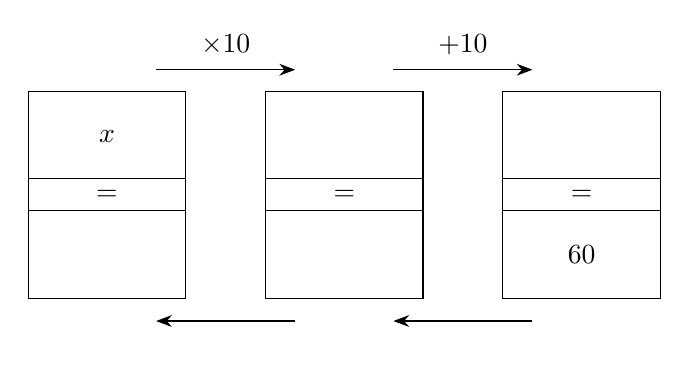
\begin{tikzpicture}[baseline={([yshift=-12pt]current bounding box.north)}]
            
        \node[backtrack] (boxA) at (0, 0) {$x$};
        \node[backtrack] (boxB) [right=1cm of boxA] {$$};
        \node[backtrack] (boxC) [right=1cm of boxB] {$$};
    
        \node[backtrackeq] (boxAeq) [below=-1pt of boxA] {$=$};
        \node[backtrackeq] (boxBeq) [below=-1pt of boxB] {$=$};
        \node[backtrackeq] (boxCeq) [below=-1pt of boxC] {$=$};
        
        \node[backtrack] (boxArev) [below=-1pt of boxAeq] {$$};
        \node[backtrack] (boxBrev) [below=-1pt of boxBeq] {$$};
        \node[backtrack] (boxCrev) [below=-1pt of boxCeq] {$60$};
         
        \node (boxAr) at ([yshift=24pt,xshift=5mm]boxA) { };
        \node (boxBl) at ([yshift=24pt,xshift=-5mm]boxB) { };
        \draw [line width=0.4pt,-{Stealth[length=2mm]}] (boxAr)  --node[backtrackstep, above=3.0pt] {$\times10$} (boxBl);
    
        \node (boxBr) at ([yshift=24pt,xshift=5mm]boxB) { };
        \node (boxCl) at ([yshift=24pt,xshift=-5mm]boxC) { };
        \draw [line width=0.4pt,-{Stealth[length=2mm]}] (boxBr)  --node[backtrackstep, above=3.0pt] {$+10$} (boxCl);
    
        \node (boxCrevl) at ([yshift=-24pt,xshift=-5mm]boxCrev) { };
        \node (boxBrevr) at ([yshift=-24pt,xshift=5mm]boxBrev) { };
        \draw [line width=0.4pt,-{Stealth[length=2mm]}] (boxCrevl)  --node[backtrackstep, below=3.0pt] {$$} (boxBrevr);
    
        \node (boxBrevl) at ([yshift=-24pt,xshift=-5mm]boxBrev) { };
        \node (boxArevr) at ([yshift=-24pt,xshift=5mm]boxArev) { };
        \draw [line width=0.4pt,-{Stealth[length=2mm]}] (boxBrevl)  --node[backtrackstep, below=3.0pt] {$$} (boxArevr);
        
    \end{tikzpicture}    
\end{equation}


\vspace{-2pt}\begin{equation}
    \begin{tikzpicture}[baseline={([yshift=-12pt]current bounding box.north)}]
            
        \node[backtrack] (boxA) at (0, 0) {$x$};
        \node[backtrack] (boxB) [right=1cm of boxA] {$$};
        \node[backtrack] (boxC) [right=1cm of boxB] {$$};
    
        \node[backtrackeq] (boxAeq) [below=-1pt of boxA] {$=$};
        \node[backtrackeq] (boxBeq) [below=-1pt of boxB] {$=$};
        \node[backtrackeq] (boxCeq) [below=-1pt of boxC] {$=$};
        
        \node[backtrack] (boxArev) [below=-1pt of boxAeq] {$$};
        \node[backtrack] (boxBrev) [below=-1pt of boxBeq] {$$};
        \node[backtrack] (boxCrev) [below=-1pt of boxCeq] {$57$};
         
        \node (boxAr) at ([yshift=24pt,xshift=5mm]boxA) { };
        \node (boxBl) at ([yshift=24pt,xshift=-5mm]boxB) { };
        \draw [line width=0.4pt,-{Stealth[length=2mm]}] (boxAr)  --node[backtrackstep, above=3.0pt] {$\times5$} (boxBl);
    
        \node (boxBr) at ([yshift=24pt,xshift=5mm]boxB) { };
        \node (boxCl) at ([yshift=24pt,xshift=-5mm]boxC) { };
        \draw [line width=0.4pt,-{Stealth[length=2mm]}] (boxBr)  --node[backtrackstep, above=3.0pt] {$+7$} (boxCl);
    
        \node (boxCrevl) at ([yshift=-24pt,xshift=-5mm]boxCrev) { };
        \node (boxBrevr) at ([yshift=-24pt,xshift=5mm]boxBrev) { };
        \draw [line width=0.4pt,-{Stealth[length=2mm]}] (boxCrevl)  --node[backtrackstep, below=3.0pt] {$$} (boxBrevr);
    
        \node (boxBrevl) at ([yshift=-24pt,xshift=-5mm]boxBrev) { };
        \node (boxArevr) at ([yshift=-24pt,xshift=5mm]boxArev) { };
        \draw [line width=0.4pt,-{Stealth[length=2mm]}] (boxBrevl)  --node[backtrackstep, below=3.0pt] {$$} (boxArevr);
        
    \end{tikzpicture}    
\end{equation}


\vspace{-2pt}\begin{equation}
    \begin{tikzpicture}[baseline={([yshift=-12pt]current bounding box.north)}]
            
        \node[backtrack] (boxA) at (0, 0) {$x$};
        \node[backtrack] (boxB) [right=1cm of boxA] {$$};
        \node[backtrack] (boxC) [right=1cm of boxB] {$$};
    
        \node[backtrackeq] (boxAeq) [below=-1pt of boxA] {$=$};
        \node[backtrackeq] (boxBeq) [below=-1pt of boxB] {$=$};
        \node[backtrackeq] (boxCeq) [below=-1pt of boxC] {$=$};
        
        \node[backtrack] (boxArev) [below=-1pt of boxAeq] {$$};
        \node[backtrack] (boxBrev) [below=-1pt of boxBeq] {$$};
        \node[backtrack] (boxCrev) [below=-1pt of boxCeq] {$17$};
         
        \node (boxAr) at ([yshift=24pt,xshift=5mm]boxA) { };
        \node (boxBl) at ([yshift=24pt,xshift=-5mm]boxB) { };
        \draw [line width=0.4pt,-{Stealth[length=2mm]}] (boxAr)  --node[backtrackstep, above=3.0pt] {$\times5$} (boxBl);
    
        \node (boxBr) at ([yshift=24pt,xshift=5mm]boxB) { };
        \node (boxCl) at ([yshift=24pt,xshift=-5mm]boxC) { };
        \draw [line width=0.4pt,-{Stealth[length=2mm]}] (boxBr)  --node[backtrackstep, above=3.0pt] {$+2$} (boxCl);
    
        \node (boxCrevl) at ([yshift=-24pt,xshift=-5mm]boxCrev) { };
        \node (boxBrevr) at ([yshift=-24pt,xshift=5mm]boxBrev) { };
        \draw [line width=0.4pt,-{Stealth[length=2mm]}] (boxCrevl)  --node[backtrackstep, below=3.0pt] {$$} (boxBrevr);
    
        \node (boxBrevl) at ([yshift=-24pt,xshift=-5mm]boxBrev) { };
        \node (boxArevr) at ([yshift=-24pt,xshift=5mm]boxArev) { };
        \draw [line width=0.4pt,-{Stealth[length=2mm]}] (boxBrevl)  --node[backtrackstep, below=3.0pt] {$$} (boxArevr);
        
    \end{tikzpicture}    
\end{equation}


\vspace{-2pt}\begin{equation}
    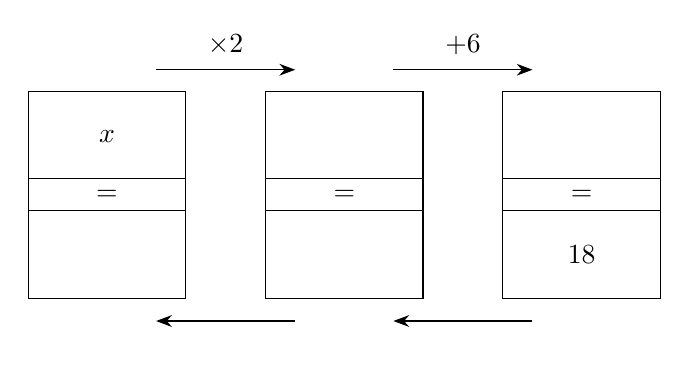
\begin{tikzpicture}[baseline={([yshift=-12pt]current bounding box.north)}]
            
        \node[backtrack] (boxA) at (0, 0) {$x$};
        \node[backtrack] (boxB) [right=1cm of boxA] {$$};
        \node[backtrack] (boxC) [right=1cm of boxB] {$$};
    
        \node[backtrackeq] (boxAeq) [below=-1pt of boxA] {$=$};
        \node[backtrackeq] (boxBeq) [below=-1pt of boxB] {$=$};
        \node[backtrackeq] (boxCeq) [below=-1pt of boxC] {$=$};
        
        \node[backtrack] (boxArev) [below=-1pt of boxAeq] {$$};
        \node[backtrack] (boxBrev) [below=-1pt of boxBeq] {$$};
        \node[backtrack] (boxCrev) [below=-1pt of boxCeq] {$18$};
         
        \node (boxAr) at ([yshift=24pt,xshift=5mm]boxA) { };
        \node (boxBl) at ([yshift=24pt,xshift=-5mm]boxB) { };
        \draw [line width=0.4pt,-{Stealth[length=2mm]}] (boxAr)  --node[backtrackstep, above=3.0pt] {$\times2$} (boxBl);
    
        \node (boxBr) at ([yshift=24pt,xshift=5mm]boxB) { };
        \node (boxCl) at ([yshift=24pt,xshift=-5mm]boxC) { };
        \draw [line width=0.4pt,-{Stealth[length=2mm]}] (boxBr)  --node[backtrackstep, above=3.0pt] {$+6$} (boxCl);
    
        \node (boxCrevl) at ([yshift=-24pt,xshift=-5mm]boxCrev) { };
        \node (boxBrevr) at ([yshift=-24pt,xshift=5mm]boxBrev) { };
        \draw [line width=0.4pt,-{Stealth[length=2mm]}] (boxCrevl)  --node[backtrackstep, below=3.0pt] {$$} (boxBrevr);
    
        \node (boxBrevl) at ([yshift=-24pt,xshift=-5mm]boxBrev) { };
        \node (boxArevr) at ([yshift=-24pt,xshift=5mm]boxArev) { };
        \draw [line width=0.4pt,-{Stealth[length=2mm]}] (boxBrevl)  --node[backtrackstep, below=3.0pt] {$$} (boxArevr);
        
    \end{tikzpicture}    
\end{equation}


\vspace{-2pt}\begin{equation}
    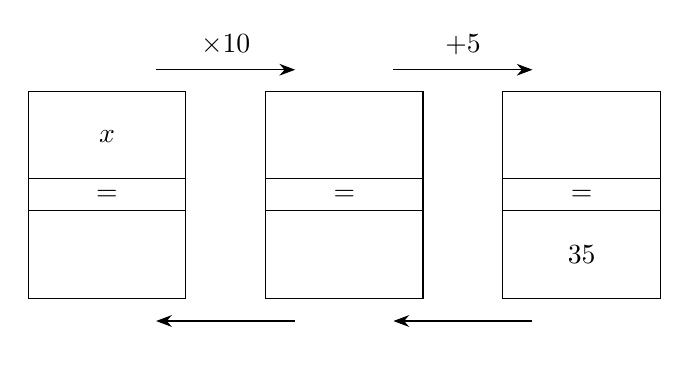
\begin{tikzpicture}[baseline={([yshift=-12pt]current bounding box.north)}]
            
        \node[backtrack] (boxA) at (0, 0) {$x$};
        \node[backtrack] (boxB) [right=1cm of boxA] {$$};
        \node[backtrack] (boxC) [right=1cm of boxB] {$$};
    
        \node[backtrackeq] (boxAeq) [below=-1pt of boxA] {$=$};
        \node[backtrackeq] (boxBeq) [below=-1pt of boxB] {$=$};
        \node[backtrackeq] (boxCeq) [below=-1pt of boxC] {$=$};
        
        \node[backtrack] (boxArev) [below=-1pt of boxAeq] {$$};
        \node[backtrack] (boxBrev) [below=-1pt of boxBeq] {$$};
        \node[backtrack] (boxCrev) [below=-1pt of boxCeq] {$35$};
         
        \node (boxAr) at ([yshift=24pt,xshift=5mm]boxA) { };
        \node (boxBl) at ([yshift=24pt,xshift=-5mm]boxB) { };
        \draw [line width=0.4pt,-{Stealth[length=2mm]}] (boxAr)  --node[backtrackstep, above=3.0pt] {$\times10$} (boxBl);
    
        \node (boxBr) at ([yshift=24pt,xshift=5mm]boxB) { };
        \node (boxCl) at ([yshift=24pt,xshift=-5mm]boxC) { };
        \draw [line width=0.4pt,-{Stealth[length=2mm]}] (boxBr)  --node[backtrackstep, above=3.0pt] {$+5$} (boxCl);
    
        \node (boxCrevl) at ([yshift=-24pt,xshift=-5mm]boxCrev) { };
        \node (boxBrevr) at ([yshift=-24pt,xshift=5mm]boxBrev) { };
        \draw [line width=0.4pt,-{Stealth[length=2mm]}] (boxCrevl)  --node[backtrackstep, below=3.0pt] {$$} (boxBrevr);
    
        \node (boxBrevl) at ([yshift=-24pt,xshift=-5mm]boxBrev) { };
        \node (boxArevr) at ([yshift=-24pt,xshift=5mm]boxArev) { };
        \draw [line width=0.4pt,-{Stealth[length=2mm]}] (boxBrevl)  --node[backtrackstep, below=3.0pt] {$$} (boxArevr);
        
    \end{tikzpicture}    
\end{equation}


\vspace{-2pt}\begin{equation}
    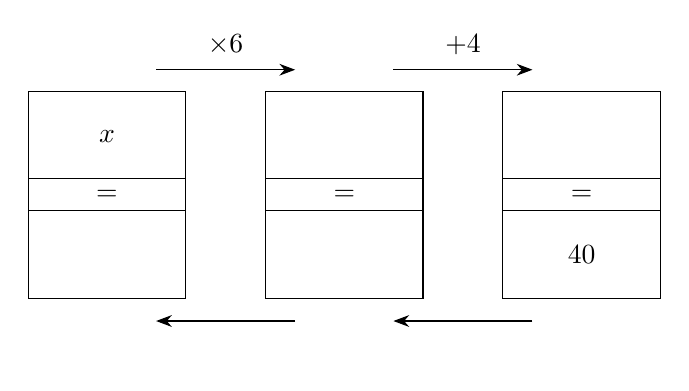
\begin{tikzpicture}[baseline={([yshift=-12pt]current bounding box.north)}]
            
        \node[backtrack] (boxA) at (0, 0) {$x$};
        \node[backtrack] (boxB) [right=1cm of boxA] {$$};
        \node[backtrack] (boxC) [right=1cm of boxB] {$$};
    
        \node[backtrackeq] (boxAeq) [below=-1pt of boxA] {$=$};
        \node[backtrackeq] (boxBeq) [below=-1pt of boxB] {$=$};
        \node[backtrackeq] (boxCeq) [below=-1pt of boxC] {$=$};
        
        \node[backtrack] (boxArev) [below=-1pt of boxAeq] {$$};
        \node[backtrack] (boxBrev) [below=-1pt of boxBeq] {$$};
        \node[backtrack] (boxCrev) [below=-1pt of boxCeq] {$40$};
         
        \node (boxAr) at ([yshift=24pt,xshift=5mm]boxA) { };
        \node (boxBl) at ([yshift=24pt,xshift=-5mm]boxB) { };
        \draw [line width=0.4pt,-{Stealth[length=2mm]}] (boxAr)  --node[backtrackstep, above=3.0pt] {$\times6$} (boxBl);
    
        \node (boxBr) at ([yshift=24pt,xshift=5mm]boxB) { };
        \node (boxCl) at ([yshift=24pt,xshift=-5mm]boxC) { };
        \draw [line width=0.4pt,-{Stealth[length=2mm]}] (boxBr)  --node[backtrackstep, above=3.0pt] {$+4$} (boxCl);
    
        \node (boxCrevl) at ([yshift=-24pt,xshift=-5mm]boxCrev) { };
        \node (boxBrevr) at ([yshift=-24pt,xshift=5mm]boxBrev) { };
        \draw [line width=0.4pt,-{Stealth[length=2mm]}] (boxCrevl)  --node[backtrackstep, below=3.0pt] {$$} (boxBrevr);
    
        \node (boxBrevl) at ([yshift=-24pt,xshift=-5mm]boxBrev) { };
        \node (boxArevr) at ([yshift=-24pt,xshift=5mm]boxArev) { };
        \draw [line width=0.4pt,-{Stealth[length=2mm]}] (boxBrevl)  --node[backtrackstep, below=3.0pt] {$$} (boxArevr);
        
    \end{tikzpicture}    
\end{equation}


\vspace{-2pt}
    \end{multicols}
\end{document}
